\documentclass{standalone}
\usepackage{tikz}
\usetikzlibrary{patterns, positioning}

\begin{document}
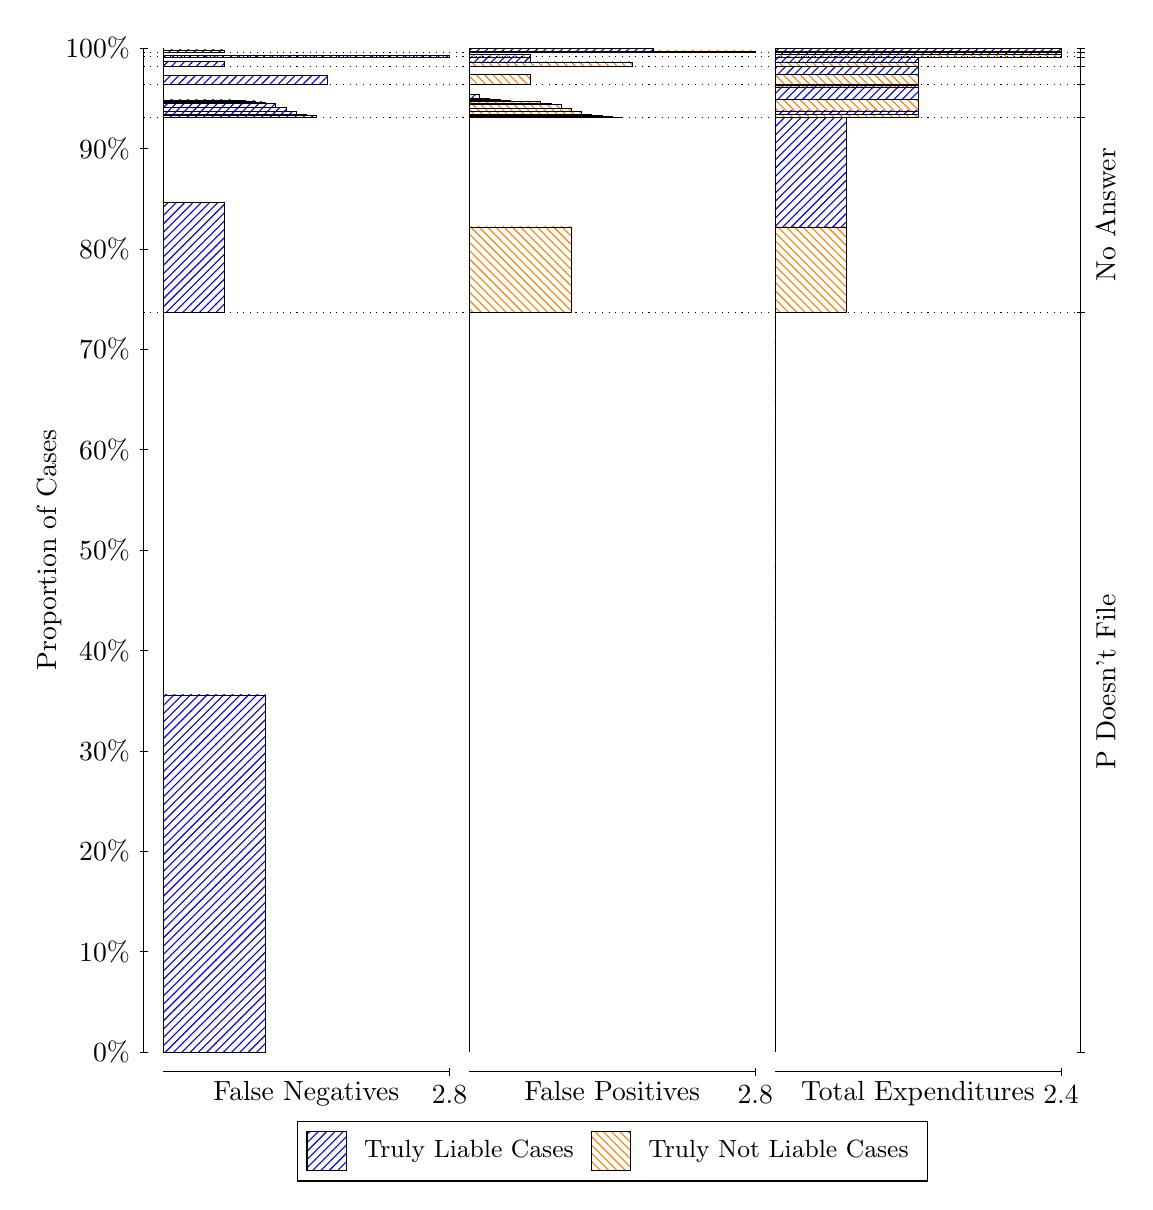
\begin{tikzpicture}
\draw[black, very thin] (1.5,1.75) -- (1.5,14.5);
\node[rotate=90, anchor=center] at (0.3, 8.125) {Proportion of Cases};
\draw[black, very thin] (1.45,1.75) -- (1.55,1.75);
\node[anchor=east] at (1.45, 1.75) {0\%};
\draw[black, very thin] (1.45,3.025) -- (1.55,3.025);
\node[anchor=east] at (1.45, 3.025) {10\%};
\draw[black, very thin] (1.45,4.3) -- (1.55,4.3);
\node[anchor=east] at (1.45, 4.3) {20\%};
\draw[black, very thin] (1.45,5.575) -- (1.55,5.575);
\node[anchor=east] at (1.45, 5.575) {30\%};
\draw[black, very thin] (1.45,6.85) -- (1.55,6.85);
\node[anchor=east] at (1.45, 6.85) {40\%};
\draw[black, very thin] (1.45,8.125) -- (1.55,8.125);
\node[anchor=east] at (1.45, 8.125) {50\%};
\draw[black, very thin] (1.45,9.4) -- (1.55,9.4);
\node[anchor=east] at (1.45, 9.4) {60\%};
\draw[black, very thin] (1.45,10.675) -- (1.55,10.675);
\node[anchor=east] at (1.45, 10.675) {70\%};
\draw[black, very thin] (1.45,11.95) -- (1.55,11.95);
\node[anchor=east] at (1.45, 11.95) {80\%};
\draw[black, very thin] (1.45,13.225) -- (1.55,13.225);
\node[anchor=east] at (1.45, 13.225) {90\%};
\draw[black, very thin] (1.45,14.5) -- (1.55,14.5);
\node[anchor=east] at (1.45, 14.5) {100\%};

\draw[black, very thin] (13.4,1.75) -- (13.4,14.5);
\draw[black, very thin] (13.35,1.75) -- (13.45,1.75);
\node[anchor=west] at (13.35, 1.75) {};
\draw[black, very thin] (13.35,11.146) -- (13.45,11.146);
\node[anchor=west] at (13.35, 11.146) {};
\draw[black, very thin] (13.35,13.619) -- (13.45,13.619);
\node[anchor=west] at (13.35, 13.619) {};
\draw[black, very thin] (13.35,14.042) -- (13.45,14.042);
\node[anchor=west] at (13.35, 14.042) {};
\draw[black, very thin] (13.35,14.269) -- (13.45,14.269);
\node[anchor=west] at (13.35, 14.269) {};
\draw[black, very thin] (13.35,14.387) -- (13.45,14.387);
\node[anchor=west] at (13.35, 14.387) {};
\draw[black, very thin] (13.35,14.441) -- (13.45,14.441);
\node[anchor=west] at (13.35, 14.441) {};
\draw[black, very thin] (13.35,14.5) -- (13.45,14.5);
\node[anchor=west] at (13.35, 14.5) {};

\draw[black, very thin, pattern color=blue, pattern=north east lines] (1.75,1.75) rectangle (3.0476,6.2858);
\draw[black, very thin, pattern color=orange, pattern=north west lines] (1.75,6.2858) rectangle (1.75,11.146);
\draw[black, very thin, pattern color=blue, pattern=north east lines] (1.75,11.146) rectangle (2.5286,12.537);
\draw[black, very thin, pattern color=orange, pattern=north west lines] (1.75,12.537) rectangle (1.75,13.619);
\draw[black, very thin, pattern color=blue, pattern=north east lines] (1.75,13.619) rectangle (3.6964,13.641);
\draw[black, very thin, pattern color=blue, pattern=north east lines] (1.75,13.641) rectangle (3.5667,13.653);
\draw[black, very thin, pattern color=blue, pattern=north east lines] (1.75,13.653) rectangle (3.4369,13.7);
\draw[black, very thin, pattern color=blue, pattern=north east lines] (1.75,13.7) rectangle (3.3071,13.75);
\draw[black, very thin, pattern color=blue, pattern=north east lines] (1.75,13.75) rectangle (3.1774,13.797);
\draw[black, very thin, pattern color=blue, pattern=north east lines] (1.75,13.797) rectangle (3.0476,13.817);
\draw[black, very thin, pattern color=blue, pattern=north east lines] (1.75,13.817) rectangle (2.9179,13.83);
\draw[black, very thin, pattern color=blue, pattern=north east lines] (1.75,13.83) rectangle (2.7881,13.837);
\draw[black, very thin, pattern color=blue, pattern=north east lines] (1.75,13.837) rectangle (2.6583,13.842);
\draw[black, very thin, pattern color=orange, pattern=north west lines] (1.75,13.842) rectangle (1.75,14.042);
\draw[black, very thin, pattern color=blue, pattern=north east lines] (1.75,14.042) rectangle (3.8262,14.148);
\draw[black, very thin, pattern color=orange, pattern=north west lines] (1.75,14.148) rectangle (1.75,14.269);
\draw[black, very thin, pattern color=blue, pattern=north east lines] (1.75,14.269) rectangle (2.5286,14.332);
\draw[black, very thin, pattern color=orange, pattern=north west lines] (1.75,14.332) rectangle (1.75,14.387);
\draw[black, very thin, pattern color=blue, pattern=north east lines] (1.75,14.387) rectangle (5.3833,14.408);
\draw[black, very thin, pattern color=orange, pattern=north west lines] (1.75,14.408) rectangle (1.75,14.441);
\draw[black, very thin, pattern color=blue, pattern=north east lines] (1.75,14.441) rectangle (2.5286,14.477);
\draw[black, very thin, pattern color=orange, pattern=north west lines] (1.75,14.477) rectangle (1.75,14.5);
\draw[black, very thin, pattern color=orange, pattern=north west lines] (5.6333,1.75) rectangle (5.6333,6.6106);
\draw[black, very thin, pattern color=blue, pattern=north east lines] (5.6333,6.6106) rectangle (5.6333,11.146);
\draw[black, very thin, pattern color=orange, pattern=north west lines] (5.6333,11.146) rectangle (6.931,12.229);
\draw[black, very thin, pattern color=blue, pattern=north east lines] (5.6333,12.229) rectangle (5.6333,13.619);
\draw[black, very thin, pattern color=orange, pattern=north west lines] (5.6333,13.619) rectangle (7.5798,13.624);
\draw[black, very thin, pattern color=orange, pattern=north west lines] (5.6333,13.624) rectangle (7.45,13.629);
\draw[black, very thin, pattern color=orange, pattern=north west lines] (5.6333,13.629) rectangle (7.3202,13.64);
\draw[black, very thin, pattern color=orange, pattern=north west lines] (5.6333,13.64) rectangle (7.1905,13.657);
\draw[black, very thin, pattern color=orange, pattern=north west lines] (5.6333,13.657) rectangle (7.0607,13.694);
\draw[black, very thin, pattern color=orange, pattern=north west lines] (5.6333,13.694) rectangle (6.931,13.734);
\draw[black, very thin, pattern color=orange, pattern=north west lines] (5.6333,13.734) rectangle (6.8012,13.782);
\draw[black, very thin, pattern color=orange, pattern=north west lines] (5.6333,13.782) rectangle (6.6714,13.795);
\draw[black, very thin, pattern color=orange, pattern=north west lines] (5.6333,13.795) rectangle (6.5417,13.82);
\draw[black, very thin, pattern color=blue, pattern=north east lines] (5.6333,13.82) rectangle (6.2821,13.825);
\draw[black, very thin, pattern color=blue, pattern=north east lines] (5.6333,13.825) rectangle (6.1524,13.831);
\draw[black, very thin, pattern color=blue, pattern=north east lines] (5.6333,13.831) rectangle (6.0226,13.845);
\draw[black, very thin, pattern color=blue, pattern=north east lines] (5.6333,13.845) rectangle (5.8929,13.864);
\draw[black, very thin, pattern color=blue, pattern=north east lines] (5.6333,13.864) rectangle (5.7631,13.911);
\draw[black, very thin, pattern color=blue, pattern=north east lines] (5.6333,13.911) rectangle (5.6333,14.042);
\draw[black, very thin, pattern color=orange, pattern=north west lines] (5.6333,14.042) rectangle (6.4119,14.163);
\draw[black, very thin, pattern color=blue, pattern=north east lines] (5.6333,14.163) rectangle (5.6333,14.269);
\draw[black, very thin, pattern color=orange, pattern=north west lines] (5.6333,14.269) rectangle (7.7095,14.324);
\draw[black, very thin, pattern color=blue, pattern=north east lines] (5.6333,14.324) rectangle (6.4119,14.387);
\draw[black, very thin, pattern color=orange, pattern=north west lines] (5.6333,14.387) rectangle (6.4119,14.42);
\draw[black, very thin, pattern color=blue, pattern=north east lines] (5.6333,14.42) rectangle (5.6333,14.441);
\draw[black, very thin, pattern color=orange, pattern=north west lines] (5.6333,14.441) rectangle (9.2667,14.464);
\draw[black, very thin, pattern color=blue, pattern=north east lines] (5.6333,14.464) rectangle (7.969,14.5);
\draw[black, very thin, pattern color=orange, pattern=north west lines] (9.5167,1.75) rectangle (9.5167,6.6106);
\draw[black, very thin, pattern color=blue, pattern=north east lines] (9.5167,6.6106) rectangle (9.5167,11.146);
\draw[black, very thin, pattern color=orange, pattern=north west lines] (9.5167,11.146) rectangle (10.425,12.229);
\draw[black, very thin, pattern color=blue, pattern=north east lines] (9.5167,12.229) rectangle (10.425,13.619);
\draw[black, very thin, pattern color=orange, pattern=north west lines] (9.5167,13.619) rectangle (11.333,13.656);
\draw[black, very thin, pattern color=blue, pattern=north east lines] (9.5167,13.656) rectangle (11.333,13.703);
\draw[black, very thin, pattern color=orange, pattern=north west lines] (9.5167,13.703) rectangle (11.333,13.851);
\draw[black, very thin, pattern color=blue, pattern=north east lines] (9.5167,13.851) rectangle (11.333,14.006);
\draw[black, very thin, pattern color=orange, pattern=north west lines] (9.5167,14.006) rectangle (11.333,14.022);
\draw[black, very thin, pattern color=blue, pattern=north east lines] (9.5167,14.022) rectangle (11.333,14.042);
\draw[black, very thin, pattern color=orange, pattern=north west lines] (9.5167,14.042) rectangle (11.333,14.163);
\draw[black, very thin, pattern color=blue, pattern=north east lines] (9.5167,14.163) rectangle (11.333,14.269);
\draw[black, very thin, pattern color=orange, pattern=north west lines] (9.5167,14.269) rectangle (11.333,14.324);
\draw[black, very thin, pattern color=blue, pattern=north east lines] (9.5167,14.324) rectangle (11.333,14.387);
\draw[black, very thin, pattern color=orange, pattern=north west lines] (9.5167,14.387) rectangle (13.15,14.42);
\draw[black, very thin, pattern color=blue, pattern=north east lines] (9.5167,14.42) rectangle (13.15,14.441);
\draw[black, very thin, pattern color=orange, pattern=north west lines] (9.5167,14.441) rectangle (13.15,14.464);
\draw[black, very thin, pattern color=blue, pattern=north east lines] (9.5167,14.464) rectangle (13.15,14.5);
\draw[black, dotted] (1.5,11.146) -- (13.4,11.146);
\draw[black, dotted] (1.5,13.619) -- (13.4,13.619);
\draw[black, dotted] (1.5,14.042) -- (13.4,14.042);
\draw[black, dotted] (1.5,14.269) -- (13.4,14.269);
\draw[black, dotted] (1.5,14.387) -- (13.4,14.387);
\draw[black, dotted] (1.5,14.441) -- (13.4,14.441);
\draw[black, very thin] (1.75,1.5) -- (5.3833,1.5);
\node[anchor=north] at (3.5667, 1.5) {False Negatives};
\draw[black, very thin] (5.3833,1.45) -- (5.3833,1.55);
\node[anchor=north] at (5.3833, 1.45) {2.8};

\draw[black, very thin] (5.6333,1.5) -- (9.2667,1.5);
\node[anchor=north] at (7.45, 1.5) {False Positives};
\draw[black, very thin] (9.2667,1.45) -- (9.2667,1.55);
\node[anchor=north] at (9.2667, 1.45) {2.8};

\draw[black, very thin] (9.5167,1.5) -- (13.15,1.5);
\node[anchor=north] at (11.333, 1.5) {Total Expenditures};
\draw[black, very thin] (13.15,1.45) -- (13.15,1.55);
\node[anchor=north] at (13.15, 1.45) {2.4};

\node[black, centered, rotate=90] at (13.72, 6.4482) {P Doesn't File};
\node[black, centered, rotate=90] at (13.72, 12.383) {No Answer};






\draw (7.449999999999999,1.5) node[draw=none] (baseCoordinate) {};
\begin{scope}[align=center]
        \matrix[scale=0.5, draw=black, below=0.5cm of baseCoordinate, nodes={draw}, column sep=0.1cm]{
            \node[rectangle, draw, minimum width=0.5cm, minimum height=0.5cm, pattern=north east lines, pattern color=blue] {}; &
            \node[draw=none, font=\small] (B) {Truly Liable Cases}; &
            \node[rectangle, draw, minimum width=0.5cm, minimum height=0.5cm, pattern=north west lines, pattern color=orange] {}; &
            \node[draw=none, font=\small] (B) {Truly Not Liable Cases}; \\
            };
\end{scope}

\end{tikzpicture}
\end{document}